% This LaTeX was auto-generated from MATLAB code.
% To make changes, update the MATLAB code and export to LaTeX again.

\documentclass{article}

\usepackage[utf8]{inputenc}
\usepackage[T1]{fontenc}
\usepackage{lmodern}
\usepackage{graphicx}
\usepackage{color}
\usepackage{hyperref}
\usepackage{amsmath}
\usepackage{amsfonts}
\usepackage{epstopdf}
\usepackage[table]{xcolor}
\usepackage{matlab}

\sloppy
\epstopdfsetup{outdir=./}
\graphicspath{ {./imuAnalysis_images/} }

\begin{document}

\matlabtitle{Rock No Rock: IMU analysis}

\begin{par}
\begin{flushleft}
Enter subject code 
\end{flushleft}
\end{par}

\begin{matlabcode}
subName = 'eg';
\end{matlabcode}

\begin{par}
\begin{flushleft}
Run subject's data LiveScript to get data table
\end{flushleft}
\end{par}

\begin{matlabcode}
run(['data_' subName '.mlx']);
\end{matlabcode}
\begin{matlabtableoutput}
{
\begin{tabular} {|c|c|c|c|c|c|c|}\hline
\mlcell{ } & \mlcell{number} & \mlcell{code} & \mlcell{sex} & \mlcell{age} & \mlcell{mass} & \mlcell{h} \\ \hline
\mlcell{1} & \mlcell{5} & \mlcell{'eg'} & \mlcell{'M'} & \mlcell{30} & \mlcell{148} & \mlcell{1.7800} \\ 
\hline
\end{tabular}
}
\end{matlabtableoutput}
\begin{matlaboutput}
listHang = 3x1    
    7.4000
   14.8000
   26.6400

Predicted maximal power output = 814.5 Watts 
Predicted optimal cadence = 102.0 rpm 
Predicted optimal hanging mass =  8.4 kg (18.5 lb) 
\end{matlaboutput}
\begin{center}
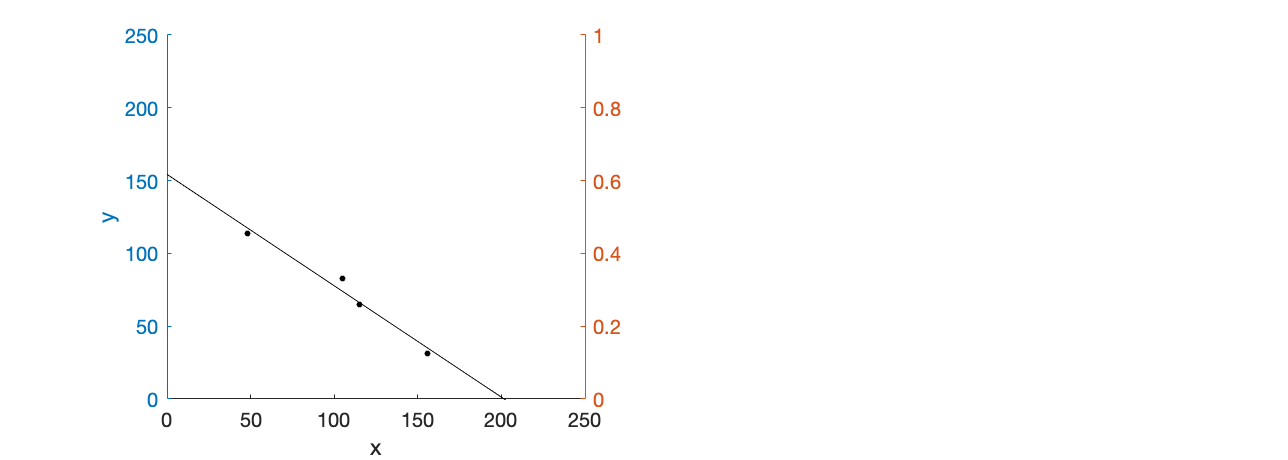
\includegraphics[width=\maxwidth{64.62619167084797em}]{figure_0.png}
\end{center}
\begin{matlaboutput}
Estimated coefficient of friction on flywheel =  1.1 
f = 
           c1: [1x1 cfit]
          gof: [1x1 struct]
     maxPower: 814.4802
       optCad: 102
      optHang: 8.3760
    maxTorque: 154.2758
         data: [4x5 table]

ans = 1x3    
     2     3     1

ans = 1x3    
     2     3     1

ans = 1x3    
     2     3     1

\end{matlaboutput}
\begin{matlabtableoutput}
{
\begin{tabular} {|c|c|c|c|c|c|c|}\hline
\mlcell{ } & \mlcell{subject} & \mlcell{condition} & \mlcell{trial} & \mlcell{hangingWeight} & \mlcell{power} & \mlcell{cadence} \\ \hline
\mlcell{1} & \mlcell{5} & \mlcell{1} & \mlcell{1} & \mlcell{17.5000} & \mlcell{908} & \mlcell{105} \\ \hline
\mlcell{2} & \mlcell{5} & \mlcell{2} & \mlcell{1} & \mlcell{17.5000} & \mlcell{787} & \mlcell{96} \\ \hline
\mlcell{3} & \mlcell{5} & \mlcell{3} & \mlcell{1} & \mlcell{17.5000} & \mlcell{808} & \mlcell{100} \\ \hline
\mlcell{4} & \mlcell{5} & \mlcell{3} & \mlcell{2} & \mlcell{17.5000} & \mlcell{829} & \mlcell{103} \\ \hline
\mlcell{5} & \mlcell{5} & \mlcell{1} & \mlcell{2} & \mlcell{17.5000} & \mlcell{859} & \mlcell{104} \\ \hline
\mlcell{6} & \mlcell{5} & \mlcell{2} & \mlcell{2} & \mlcell{17.5000} & \mlcell{683} & \mlcell{92} \\ \hline
\mlcell{7} & \mlcell{5} & \mlcell{2} & \mlcell{3} & \mlcell{17.5000} & \mlcell{774} & \mlcell{99} \\ \hline
\mlcell{8} & \mlcell{5} & \mlcell{3} & \mlcell{3} & \mlcell{17.5000} & \mlcell{821} & \mlcell{103} \\ \hline
\mlcell{9} & \mlcell{5} & \mlcell{1} & \mlcell{3} & \mlcell{17.5000} & \mlcell{899} & \mlcell{106} \\ 
\hline
\end{tabular}
}
{
\begin{tabular} {|c|c|c|c|c|}\hline
\mlcell{ } & \mlcell{condition} & \mlcell{GroupCount} & \mlcell{mean\_power} & \mlcell{mean\_cadence} \\ \hline
\mlcell{1} & \mlcell{1} & \mlcell{3} & \mlcell{888.6667} & \mlcell{105.0000} \\ \hline
\mlcell{2} & \mlcell{2} & \mlcell{3} & \mlcell{748.0000} & \mlcell{95.6667} \\ \hline
\mlcell{3} & \mlcell{3} & \mlcell{3} & \mlcell{819.3333} & \mlcell{102.0000} \\ 
\hline
\end{tabular}
}
{
\begin{tabular} {|c|c|c|c|c|}\hline
\mlcell{ } & \mlcell{condition} & \mlcell{GroupCount} & \mlcell{std\_power} & \mlcell{std\_cadence} \\ \hline
\mlcell{1} & \mlcell{1} & \mlcell{3} & \mlcell{26.0832} & \mlcell{1.0000} \\ \hline
\mlcell{2} & \mlcell{2} & \mlcell{3} & \mlcell{56.6657} & \mlcell{3.5119} \\ \hline
\mlcell{3} & \mlcell{3} & \mlcell{3} & \mlcell{10.5987} & \mlcell{1.7321} \\ 
\hline
\end{tabular}
}
\end{matlabtableoutput}
\begin{matlaboutput}
Warning: Missing required file. Assigning NaN to lean angle.
Warning: Column headers from the file were modified to make them valid MATLAB identifiers before creating variable names for the table. The original column headers are saved in the VariableDescriptions property.
Set 'PreserveVariableNames' to true to use the original column headers as table variable names.
Warning: Column headers from the file were modified to make them valid MATLAB identifiers before creating variable names for the table. The original column headers are saved in the VariableDescriptions property.
Set 'PreserveVariableNames' to true to use the original column headers as table variable names.
Warning: Column headers from the file were modified to make them valid MATLAB identifiers before creating variable names for the table. The original column headers are saved in the VariableDescriptions property.
Set 'PreserveVariableNames' to true to use the original column headers as table variable names.
Warning: Column headers from the file were modified to make them valid MATLAB identifiers before creating variable names for the table. The original column headers are saved in the VariableDescriptions property.
Set 'PreserveVariableNames' to true to use the original column headers as table variable names.
Warning: Column headers from the file were modified to make them valid MATLAB identifiers before creating variable names for the table. The original column headers are saved in the VariableDescriptions property.
Set 'PreserveVariableNames' to true to use the original column headers as table variable names.
Warning: Column headers from the file were modified to make them valid MATLAB identifiers before creating variable names for the table. The original column headers are saved in the VariableDescriptions property.
Set 'PreserveVariableNames' to true to use the original column headers as table variable names.
Warning: Column headers from the file were modified to make them valid MATLAB identifiers before creating variable names for the table. The original column headers are saved in the VariableDescriptions property.
Set 'PreserveVariableNames' to true to use the original column headers as table variable names.
Warning: Column headers from the file were modified to make them valid MATLAB identifiers before creating variable names for the table. The original column headers are saved in the VariableDescriptions property.
Set 'PreserveVariableNames' to true to use the original column headers as table variable names.
Warning: Column headers from the file were modified to make them valid MATLAB identifiers before creating variable names for the table. The original column headers are saved in the VariableDescriptions property.
Set 'PreserveVariableNames' to true to use the original column headers as table variable names.
Warning: Column headers from the file were modified to make them valid MATLAB identifiers before creating variable names for the table. The original column headers are saved in the VariableDescriptions property.
Set 'PreserveVariableNames' to true to use the original column headers as table variable names.
Warning: Column headers from the file were modified to make them valid MATLAB identifiers before creating variable names for the table. The original column headers are saved in the VariableDescriptions property.
Set 'PreserveVariableNames' to true to use the original column headers as table variable names.
Warning: Column headers from the file were modified to make them valid MATLAB identifiers before creating variable names for the table. The original column headers are saved in the VariableDescriptions property.
Set 'PreserveVariableNames' to true to use the original column headers as table variable names.
Warning: Column headers from the file were modified to make them valid MATLAB identifiers before creating variable names for the table. The original column headers are saved in the VariableDescriptions property.
Set 'PreserveVariableNames' to true to use the original column headers as table variable names.
Warning: Column headers from the file were modified to make them valid MATLAB identifiers before creating variable names for the table. The original column headers are saved in the VariableDescriptions property.
Set 'PreserveVariableNames' to true to use the original column headers as table variable names.
Warning: Column headers from the file were modified to make them valid MATLAB identifiers before creating variable names for the table. The original column headers are saved in the VariableDescriptions property.
Set 'PreserveVariableNames' to true to use the original column headers as table variable names.
Warning: Column headers from the file were modified to make them valid MATLAB identifiers before creating variable names for the table. The original column headers are saved in the VariableDescriptions property.
Set 'PreserveVariableNames' to true to use the original column headers as table variable names.
\end{matlaboutput}
\begin{matlabtableoutput}
{
\begin{tabular} {|c|c|c|c|}\hline
\mlcell{ } & \mlcell{condition} & \mlcell{GroupCount} & \mlcell{Fun\_lean} \\ \hline
\mlcell{1} & \mlcell{1} & \mlcell{3} & \mlcell{11.6917} \\ \hline
\mlcell{2} & \mlcell{2} & \mlcell{3} & \mlcell{2.3604} \\ \hline
\mlcell{3} & \mlcell{3} & \mlcell{3} & \mlcell{1.0629} \\ 
\hline
\end{tabular}
}
{
\begin{tabular} {|c|c|c|c|}\hline
\mlcell{ } & \mlcell{condition} & \mlcell{GroupCount} & \mlcell{Fun\_lean} \\ \hline
\mlcell{1} & \mlcell{1} & \mlcell{3} & \mlcell{2.2146} \\ \hline
\mlcell{2} & \mlcell{2} & \mlcell{3} & \mlcell{0.6929} \\ \hline
\mlcell{3} & \mlcell{3} & \mlcell{3} & \mlcell{0.1763} \\ 
\hline
\end{tabular}
}
\end{matlabtableoutput}
\begin{matlabcode}
clc;close all
clearvars -except T T_ subName
\end{matlabcode}

\begin{par}
\begin{flushleft}
Enter trial name
\end{flushleft}
\end{par}

\begin{matlabcode}
condition = 2;
trial = 2;
trialName = ['0',num2str(condition),'0',num2str(trial)];
\end{matlabcode}

\begin{par}
\begin{flushleft}
Load Garmin data file into table
\end{flushleft}
\end{par}

\begin{matlabcode}
filePath = '/Users/rosswilkinson/Google Drive/projects/rock-no-rock/data/';
fileName = [subName '_' trialName '_power'];
tP = readtable([filePath fileName]);
\end{matlabcode}

\begin{par}
\begin{flushleft}
Load IMU data file for crank
\end{flushleft}
\end{par}

\begin{matlabcode}
filePath = '/Users/rosswilkinson/Google Drive/projects/rock-no-rock/data/';
fileName = [subName '_' trialName '_crank'];
tC = readtable([filePath fileName]);
\end{matlabcode}
\begin{matlaboutput}
Warning: Column headers from the file were modified to make them valid MATLAB identifiers before creating variable names for the table. The original column headers are saved in the VariableDescriptions property.
Set 'PreserveVariableNames' to true to use the original column headers as table variable names.
\end{matlaboutput}

\begin{par}
\begin{flushleft}
Load IMU data file for frame
\end{flushleft}
\end{par}

\begin{matlabcode}
filePath = '/Users/rosswilkinson/Google Drive/projects/rock-no-rock/data/';
fileName = [subName '_' trialName '_frame'];
tF = readtable([filePath fileName]);
\end{matlabcode}
\begin{matlaboutput}
Warning: Column headers from the file were modified to make them valid MATLAB identifiers before creating variable names for the table. The original column headers are saved in the VariableDescriptions property.
Set 'PreserveVariableNames' to true to use the original column headers as table variable names.
\end{matlaboutput}

\begin{par}
\begin{flushleft}
Sync Garmin and IMU data
\end{flushleft}
\end{par}

\begin{itemize}
\setlength{\itemsep}{-1ex}
   \item{\begin{flushleft} convert imu accelerations into resultant acceleration \end{flushleft}}
\end{itemize}

\begin{matlabcode}
x = tC.accel_x_m_s2_; % vertical axis
y = tC.accel_y_m_s2_;
z = tC.accel_z_m_s2_;
tC.accel_res = sqrt(x.^2 + y.^2 + z.^2);
x = tF.accel_x_m_s2_; % vertical axis
y = tF.accel_y_m_s2_;
z = tF.accel_z_m_s2_;
tF.accel_res = sqrt(x.^2 + y.^2 + z.^2);
\end{matlabcode}

\begin{par}
\begin{flushleft}
Find sync spike in crank and frame IMU
\end{flushleft}
\end{par}

\begin{matlabcode}
[~,syncC] = findpeaks(tC.accel_res,'minPeakHeight',50,"NPeaks",1);
[~,syncF] = findpeaks(tF.accel_res,'minPeakHeight',50,"NPeaks",1);
\end{matlabcode}

\begin{par}
\begin{flushleft}
Crop signals to sync spike
\end{flushleft}
\end{par}

\begin{matlabcode}
tC_ = tC(syncC:end,:);
tF_ = tF(syncF:end,:);
tC_.timestamp = tC_.timestamp - tC_.timestamp(1);
tF_.timestamp = tF_.timestamp - tF_.timestamp(1);
\end{matlabcode}

\begin{par}
\begin{flushleft}
Lowpass filter acceleration signal of x axis (vertical axis)
\end{flushleft}
\end{par}

\begin{matlabcode}
freq = 500;
pass = 2;
tC_.accel_x_m_s2_ = lowpass(tC_.accel_x_m_s2_,pass,freq);
tF_.accel_y_m_s2_ = lowpass(tF_.accel_y_m_s2_,pass,freq);
\end{matlabcode}

\begin{par}
\begin{flushleft}
Interpolate power data to match IMU sampling frequency
\end{flushleft}
\end{par}

\begin{matlabcode}
x = 0:height(tP)-1;
v = table2array(tP);
xq = 0:1/500:height(tP)-1;
temp = interp1(x',v,xq',"linear");
tP_ = array2table(temp,"VariableNames",tP.Properties.VariableNames);
\end{matlabcode}

\begin{par}
\begin{flushleft}
Crop all signals to when power is being produced
\end{flushleft}
\end{par}

\begin{matlabcode}
k = tP_.watts > 0;
t1 = min(tP_.secs(k));
t2 = max(tP_.secs(k));

tP_ = tP_(k,:);
tC_ = tC_(tC_.timestamp > t1 & tC_.timestamp < t2,:);
tF_ = tF_(tF_.timestamp > t1 & tF_.timestamp < t2,:);
\end{matlabcode}

\begin{par}
\begin{flushleft}
Differentiate acceleration in y-axis to arc displacement
\end{flushleft}
\end{par}

\begin{matlabcode}
dt = 1/500;
acc = tF_.accel_y_m_s2_;
vel = diff(acc)*dt;
pos = interp1(1:length(vel)-1,diff(vel)*dt,1:length(acc));
\end{matlabcode}

\begin{par}
\begin{flushleft}
Convert frame acceleration signals to angle
\end{flushleft}
\end{par}

\begin{matlabcode}
r = 0.53; % height of IMU above pivot in meters
tF_.theta = rad2deg(pos ./ r)';
\end{matlabcode}

\begin{par}
\begin{flushleft}
Find peaks in crank signal
\end{flushleft}
\end{par}

\begin{matlabcode}
[~,locs] = findpeaks(tC_.accel_x_m_s2_,"MinPeakProminence",5,"MinPeakDistance",150);
\end{matlabcode}

\begin{par}
\begin{flushleft}
Calculate range of bicycle lean during each crank cycle
\end{flushleft}
\end{par}

\begin{matlabcode}
for i = 1:numel(locs)-1
    leanRange(i) = range(tF_.theta(locs(i):locs(i+1)));
end
leanRange
\end{matlabcode}
\begin{matlaboutput}
leanRange = 1x4    
1.0e+-4 *

    0.3972    0.3691    0.3330    0.3016

\end{matlaboutput}
\begin{matlabcode}
T_.leanAngle(k) = max(leanRange);
\end{matlabcode}
\begin{matlaboutput}
Warning: The assignment added rows to the table, but did not assign values to all of the table's existing variables. Those variables are extended with rows containing default values.
\end{matlaboutput}

\begin{par}
\begin{flushleft}
Store peak lean angle in subject data table
\end{flushleft}
\end{par}

\begin{matlabcode}
k = T_.condition == condition & T_.trial == trial;
\end{matlabcode}

\begin{par}
\begin{flushleft}
Plot power, frame angle, and crank accel.
\end{flushleft}
\end{par}

\begin{matlabcode}
subplot(311)
plot(tP_.secs,tP_.watts)
subplot(312)
plot(tC_.timestamp,tC_.accel_x_m_s2_)
subplot(313)
plot(tF_.timestamp,tF_.theta)
\end{matlabcode}
\begin{center}
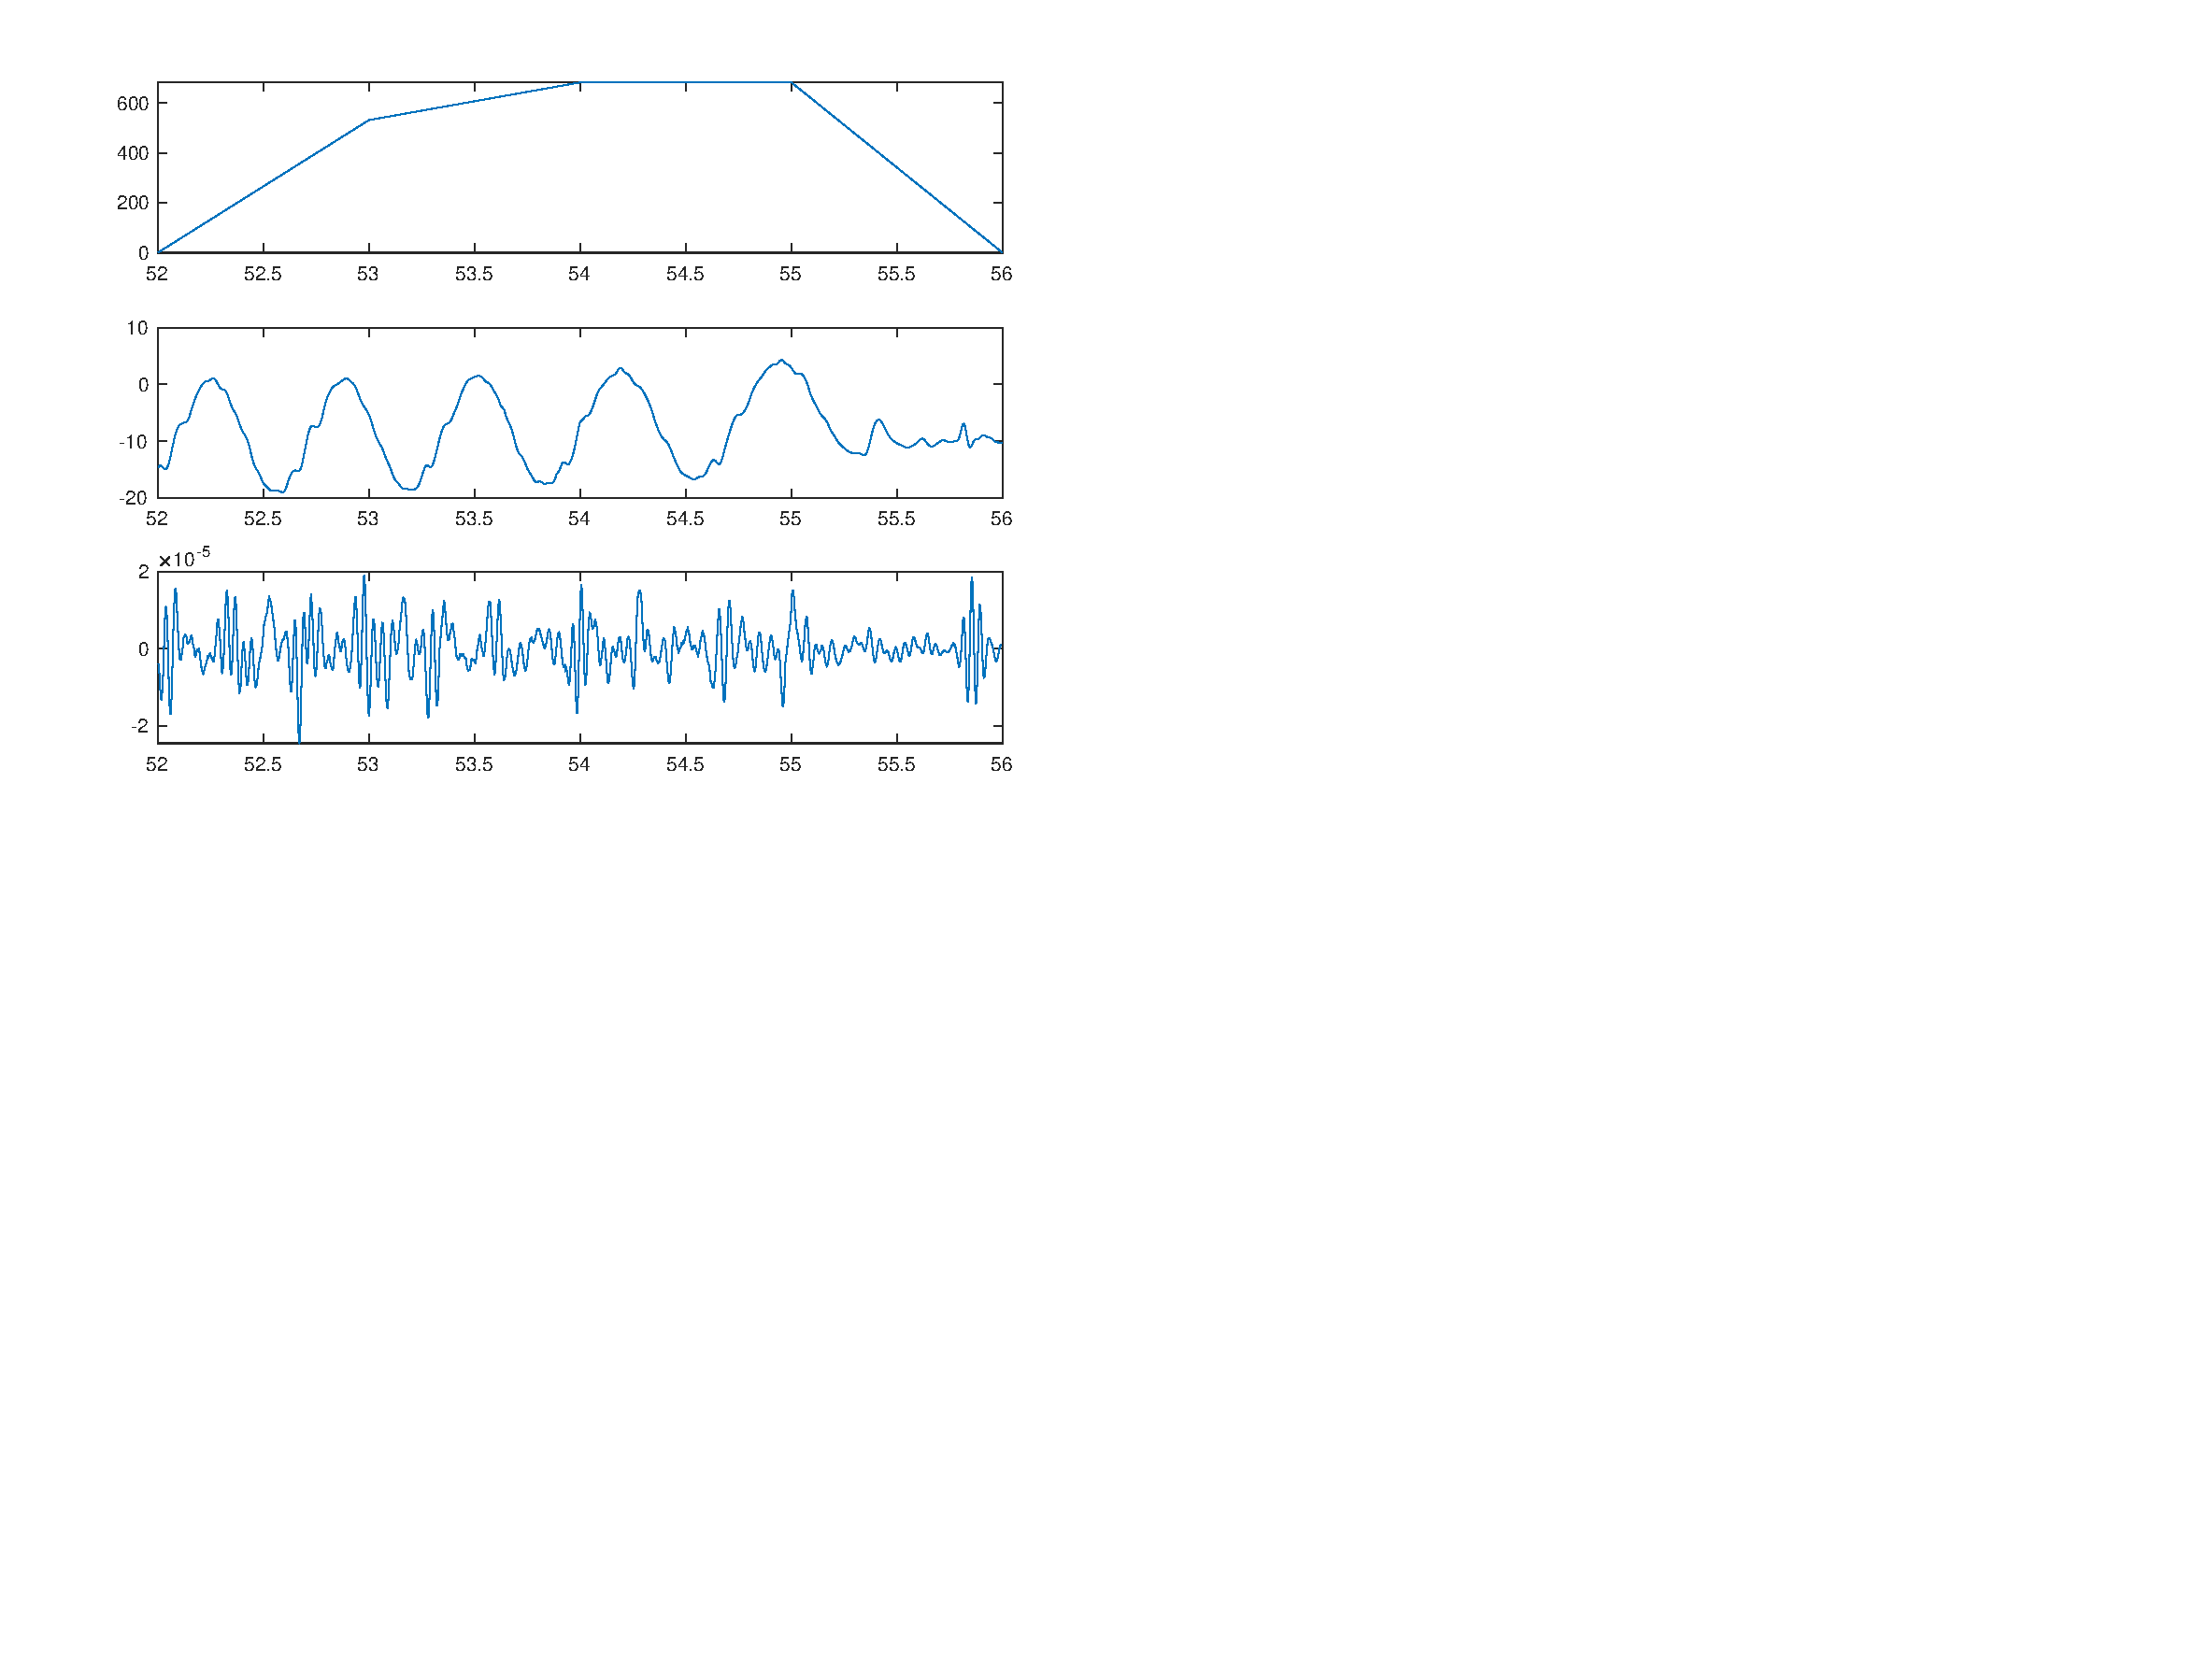
\includegraphics[width=\maxwidth{56.196688409433015em}]{figure_1.eps}
\end{center}
\begin{matlabcode}

\end{matlabcode}

\end{document}
